% !TEX root = ../../main.tex
% File: part2/chapters1/chap1_3.tex

\section{Làm sạch, Tiền xử lý và Gán nhãn Dữ liệu}
\label{sec:data_cleaning_labeling}

Dữ liệu thô thu thập được từ thế giới thực thường rất "bẩn": đầy lỗi chính tả, các ký tự lạ, thẻ HTML, và thiếu cấu trúc. Giai đoạn làm sạch, tiền xử lý và gán nhãn là quá trình biến mớ dữ liệu hỗn độn này thành một tài sản quý giá, sẵn sàng cho việc huấn luyện mô hình. Đây thường là giai đoạn tốn nhiều thời gian và công sức nhất, nhưng cũng là giai đoạn mang lại lợi tức đầu tư (ROI) cao nhất.

\subsection{Thao tác Dữ liệu quy mô lớn: Pandas, NumPy, và Polars}
\label{ssec:data_manipulation_tools}
Khi làm việc với các bộ dữ liệu văn bản lớn (từ hàng trăm nghìn đến hàng triệu dòng), việc sử dụng các cấu trúc dữ liệu cơ bản của Python (như list hay dict) sẽ trở nên rất chậm chạp. Các thư viện tính toán hiệu năng cao là không thể thiếu.

\paragraph{NumPy}
Là thư viện nền tảng cho tính toán khoa học trong Python. Nó cung cấp đối tượng mảng đa chiều `ndarray` mạnh mẽ, các phép toán tuyến tính và các hàm toán học hiệu quả. Mặc dù không trực tiếp xử lý văn bản, NumPy là "xương sống" của các thư viện khác như Pandas.

\paragraph{Pandas}
Là công cụ tiêu chuẩn trong khoa học dữ liệu để thao tác và phân tích dữ liệu dạng bảng.
\begin{itemize}
    \item \textbf{Cấu trúc dữ liệu chính:} `DataFrame`, một cấu trúc dữ liệu 2 chiều giống như một bảng tính hoặc một bảng SQL, với các hàng và các cột có nhãn.
    \item \textbf{Điểm mạnh:} Cung cấp một API cực kỳ phong phú và linh hoạt để:
        \begin{itemize}
            \item Đọc và ghi nhiều định dạng file (CSV, Excel, JSON, Parquet...).
            \item Lọc, chọn, và truy vấn dữ liệu một cách mạnh mẽ.
            \item Xử lý các giá trị bị thiếu (missing values).
            \item Áp dụng các hàm tùy chỉnh lên từng hàng hoặc cột để làm sạch và tiền xử lý văn bản.
            \item Gộp (merge) và nối (join) các bảng dữ liệu khác nhau.
        \end{itemize}
    \item \textbf{Hạn chế:} Pandas hoạt động trên một lõi CPU duy nhất và tải toàn bộ dữ liệu vào bộ nhớ RAM. Với các bộ dữ liệu cực lớn (hàng chục gigabyte), nó có thể trở nên chậm hoặc gây lỗi tràn bộ nhớ.
\end{itemize}

\paragraph{Polars: Một sự thay thế Hiện đại và Nhanh hơn}
Polars là một thư viện DataFrame mới hơn, được viết bằng Rust, và được thiết kế để giải quyết các hạn chế của Pandas.
\begin{itemize}
    \item \textbf{Điểm mạnh chính:}
        \begin{itemize}
            \item \textbf{Thực thi song song (Parallel Execution):} Polars có thể tự động tận dụng tất cả các lõi CPU có sẵn trên máy của bạn, giúp các phép toán nhanh hơn đáng kể.
            \item \textbf{Tối ưu hóa Truy vấn (Query Optimization):} Nó có một bộ tối ưu hóa truy vấn thông minh, có thể sắp xếp lại và kết hợp các phép toán để thực thi một cách hiệu quả nhất (lazy execution).
            \item \textbf{Hiệu quả về bộ nhớ:} Được thiết kế để xử lý các bộ dữ liệu lớn hơn RAM của máy.
        \end{itemize}
    \item \textbf{Khi nào nên dùng Polars?} Khi bạn làm việc với các bộ dữ liệu lớn và thấy rằng Pandas đang trở thành một "nút thắt cổ chai" về hiệu năng.
\end{itemize}

\subsection{Gán nhãn Dữ liệu: Từ Thủ công đến Tự động}
\label{ssec:data_labeling_methods}
Gán nhãn là quá trình thêm thông tin giám sát vào dữ liệu. Đây là một bước cực kỳ quan trọng và tốn kém cho các bài toán học có giám sát.

\subsubsection{Công cụ Gán nhãn Thủ công: Label Studio}
\begin{itemize}
    \item \textbf{Mục đích:} Cung cấp một giao diện người dùng trực quan để con người có thể gán nhãn dữ liệu một cách hiệu quả và nhất quán.
    \item \textbf{Label Studio là gì?} Là một công cụ gán nhãn dữ liệu mã nguồn mở và cực kỳ linh hoạt.
    \item \textbf{Các tính năng chính:}
        \begin{itemize}
            \item Hỗ trợ rất nhiều loại dữ liệu (văn bản, ảnh, âm thanh, video) và nhiều loại tác vụ NLP (phân loại, NER, trích xuất quan hệ).
            \item Giao diện có thể tùy chỉnh cao.
            \item Hỗ trợ làm việc nhóm, cho phép nhiều người cùng gán nhãn và quản lý chất lượng.
            \item Tích hợp với các mô hình học máy để "gán nhãn bán tự động" (semi-automated labeling), nơi mô hình đưa ra gợi ý và con người chỉ cần sửa lại.
        \end{itemize}
\end{itemize}
\begin{center}
    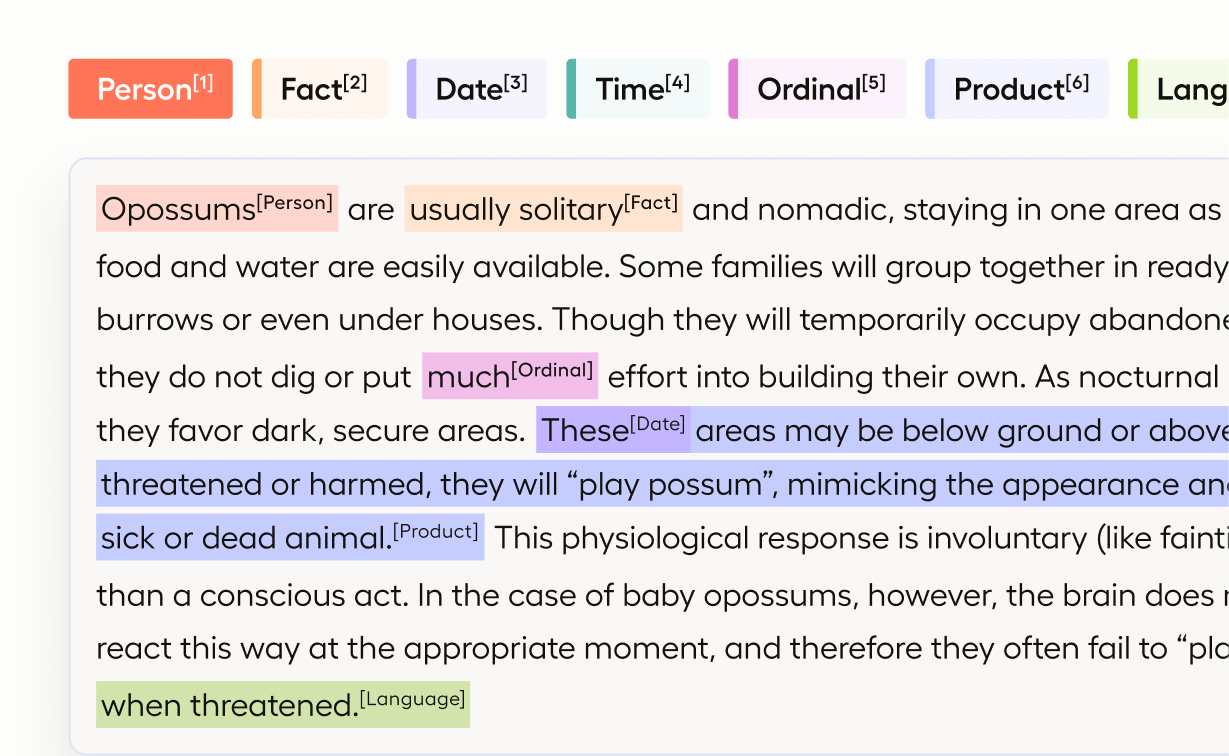
\includegraphics[width=0.8\textwidth]{label_studio_ner.png}
    \captionof{figure}{Giao diện gán nhãn Nhận dạng Thực thể Tên (NER) trong Label Studio.}
    \label{fig:label_studio_ner}
\end{center}

\subsubsection{Gán nhãn có Lập trình: Snorkel và Weak Supervision}
\begin{itemize}
    \item \textbf{Vấn đề:} Gán nhãn thủ công hàng triệu điểm dữ liệu là bất khả thi.
    \item \textbf{Tư duy của Weak Supervision:} Thay vì gán nhãn từng điểm dữ liệu một, hãy để các chuyên gia lĩnh vực (Subject Matter Experts - SMEs) viết ra các \textbf{hàm gán nhãn (Labeling Functions - LFs)} -- các quy tắc, heuristics, hoặc các mô hình đơn giản để gán nhãn dữ liệu một cách tự động nhưng có thể "nhiễu".
    \item \textbf{Snorkel là gì?} Là một framework mã nguồn mở để xây dựng các bộ dữ liệu huấn luyện bằng cách sử dụng weak supervision.
    \item \textbf{Cơ chế hoạt động:}
        \begin{enumerate}
            \item \textbf{Viết các Hàm gán nhãn (LFs):} Người dùng viết nhiều LFs. Ví dụ, để phát hiện email spam, các LFs có thể là: "Nếu email chứa từ 'khuyến mãi', gán nhãn SPAM", "Nếu email đến từ một địa chỉ trong danh bạ, gán nhãn NOT\_SPAM", "Sử dụng một mô hình Naive Bayes đơn giản để gán nhãn".
            \item \textbf{Mô hình Sinh (Generative Model):} Snorkel sẽ phân tích đầu ra của tất cả các LFs trên dữ liệu không nhãn. Nó sẽ học cách ước tính độ chính xác và sự tương quan giữa các LFs, ngay cả khi chúng mâu thuẫn với nhau.
            \item \textbf{Tạo nhãn xác suất:} Dựa trên những gì đã học, mô hình sinh sẽ kết hợp các tín hiệu yếu từ các LFs để tạo ra một nhãn xác suất (probabilistic label) duy nhất cho mỗi điểm dữ liệu.
            \item \textbf{Huấn luyện Mô hình cuối:} Các nhãn xác suất này sau đó được sử dụng để huấn luyện một mô hình phân biệt mạnh mẽ cuối cùng (ví dụ: RoBERTa).
        \end{enumerate}
    \item \textbf{Lợi ích:} Cho phép tạo ra các bộ dữ liệu huấn luyện quy mô lớn một cách nhanh chóng bằng cách tận dụng kiến thức chuyên môn thay vì công sức gán nhãn thủ công.
\end{itemize}

\subsubsection{Sử dụng LLM để Sinh và Gán nhãn Dữ liệu}
Đây là một mô hình mới nổi, tận dụng sức mạnh của các LLM lớn như GPT-4.
\begin{itemize}
    \item \textbf{Few-shot Labeling:} Cung cấp cho LLM một chỉ dẫn rõ ràng và một vài ví dụ (few-shot examples) về cách gán nhãn. Sau đó, yêu cầu nó gán nhãn cho hàng nghìn điểm dữ liệu mới. Cách này nhanh và cho chất lượng đáng kinh ngạc.
    \item \textbf{Data Generation:} LLM không chỉ có thể gán nhãn, mà còn có thể \textbf{sinh ra} các mẫu dữ liệu hoàn toàn mới. Ví dụ, để huấn luyện một mô hình phát hiện ý định, bạn có thể yêu cầu LLM: "Hãy sinh ra 20 cách khác nhau mà một người dùng có thể hỏi về tình trạng đơn hàng".
    \item \textbf{Cảnh báo:} Dữ liệu do LLM tạo ra có thể thiếu sự đa dạng và chứa các thiên vị (biases) của chính LLM đó. Cần phải kiểm tra và lọc kỹ lưỡng.
\end{itemize}

\subsection{Xử lý Dữ liệu Mất cân bằng (Handling Imbalanced Data)}
\label{ssec:imbalanced_data}
\begin{itemize}
    \item \textbf{Vấn đề:} Trong nhiều bài toán thực tế (phát hiện gian lận, chẩn đoán bệnh hiếm), số lượng mẫu của một lớp (lớp thiểu số - minority class) ít hơn rất nhiều so với các lớp khác (lớp đa số - majority class). Một mô hình được huấn luyện trên dữ liệu này có thể chỉ đơn giản là học cách "luôn dự đoán lớp đa số" để đạt độ chính xác cao, nhưng lại hoàn toàn vô dụng.
    \item \textbf{Các kỹ thuật xử lý:}
        \begin{itemize}
            \item \textbf{Lấy mẫu lại (Resampling):}
                \begin{itemize}
                    \item \textbf{Under-sampling:} Xóa bớt các mẫu từ lớp đa số. Có nguy cơ làm mất thông tin.
                    \item \textbf{Over-sampling:} Tạo ra các bản sao của các mẫu từ lớp thiểu số. Có nguy cơ gây quá khớp (overfitting).
                    \item \textbf{SMOTE (Synthetic Minority Over-sampling Technique):} Một kỹ thuật over-sampling thông minh hơn, tạo ra các mẫu "tổng hợp" mới cho lớp thiểu số bằng cách nội suy giữa các mẫu hiện có.
                \end{itemize}
            \item \textbf{Sử dụng Trọng số Lớp (Class Weights):} Trong quá trình huấn luyện, điều chỉnh hàm mất mát để "phạt" nặng hơn các lỗi mắc phải trên lớp thiểu số. Hầu hết các framework học máy đều hỗ trợ tham số `class\_weight`.
            \item \textbf{Thay đổi Metric Đánh giá:} Thay vì dùng `Accuracy`, hãy tập trung vào các metric như `F1-score`, `Precision-Recall Curve (PRC)`, hoặc `AUC-ROC` vốn ít bị ảnh hưởng bởi sự mất cân bằng.
        \end{itemize}
\end{itemize}
Việc lựa chọn kỹ thuật phù hợp phụ thuộc vào đặc điểm cụ thể của bộ dữ liệu và bài toán.